% Options for packages loaded elsewhere
\PassOptionsToPackage{unicode}{hyperref}
\PassOptionsToPackage{hyphens}{url}
\PassOptionsToPackage{dvipsnames,svgnames,x11names}{xcolor}
%
\documentclass[
  letterpaper,
  DIV=11,
  numbers=noendperiod]{scrreprt}

\usepackage{amsmath,amssymb}
\usepackage{iftex}
\ifPDFTeX
  \usepackage[T1]{fontenc}
  \usepackage[utf8]{inputenc}
  \usepackage{textcomp} % provide euro and other symbols
\else % if luatex or xetex
  \usepackage{unicode-math}
  \defaultfontfeatures{Scale=MatchLowercase}
  \defaultfontfeatures[\rmfamily]{Ligatures=TeX,Scale=1}
\fi
\usepackage{lmodern}
\ifPDFTeX\else  
    % xetex/luatex font selection
\fi
% Use upquote if available, for straight quotes in verbatim environments
\IfFileExists{upquote.sty}{\usepackage{upquote}}{}
\IfFileExists{microtype.sty}{% use microtype if available
  \usepackage[]{microtype}
  \UseMicrotypeSet[protrusion]{basicmath} % disable protrusion for tt fonts
}{}
\makeatletter
\@ifundefined{KOMAClassName}{% if non-KOMA class
  \IfFileExists{parskip.sty}{%
    \usepackage{parskip}
  }{% else
    \setlength{\parindent}{0pt}
    \setlength{\parskip}{6pt plus 2pt minus 1pt}}
}{% if KOMA class
  \KOMAoptions{parskip=half}}
\makeatother
\usepackage{xcolor}
\setlength{\emergencystretch}{3em} % prevent overfull lines
\setcounter{secnumdepth}{5}
% Make \paragraph and \subparagraph free-standing
\makeatletter
\ifx\paragraph\undefined\else
  \let\oldparagraph\paragraph
  \renewcommand{\paragraph}{
    \@ifstar
      \xxxParagraphStar
      \xxxParagraphNoStar
  }
  \newcommand{\xxxParagraphStar}[1]{\oldparagraph*{#1}\mbox{}}
  \newcommand{\xxxParagraphNoStar}[1]{\oldparagraph{#1}\mbox{}}
\fi
\ifx\subparagraph\undefined\else
  \let\oldsubparagraph\subparagraph
  \renewcommand{\subparagraph}{
    \@ifstar
      \xxxSubParagraphStar
      \xxxSubParagraphNoStar
  }
  \newcommand{\xxxSubParagraphStar}[1]{\oldsubparagraph*{#1}\mbox{}}
  \newcommand{\xxxSubParagraphNoStar}[1]{\oldsubparagraph{#1}\mbox{}}
\fi
\makeatother


\providecommand{\tightlist}{%
  \setlength{\itemsep}{0pt}\setlength{\parskip}{0pt}}\usepackage{longtable,booktabs,array}
\usepackage{calc} % for calculating minipage widths
% Correct order of tables after \paragraph or \subparagraph
\usepackage{etoolbox}
\makeatletter
\patchcmd\longtable{\par}{\if@noskipsec\mbox{}\fi\par}{}{}
\makeatother
% Allow footnotes in longtable head/foot
\IfFileExists{footnotehyper.sty}{\usepackage{footnotehyper}}{\usepackage{footnote}}
\makesavenoteenv{longtable}
\usepackage{graphicx}
\makeatletter
\def\maxwidth{\ifdim\Gin@nat@width>\linewidth\linewidth\else\Gin@nat@width\fi}
\def\maxheight{\ifdim\Gin@nat@height>\textheight\textheight\else\Gin@nat@height\fi}
\makeatother
% Scale images if necessary, so that they will not overflow the page
% margins by default, and it is still possible to overwrite the defaults
% using explicit options in \includegraphics[width, height, ...]{}
\setkeys{Gin}{width=\maxwidth,height=\maxheight,keepaspectratio}
% Set default figure placement to htbp
\makeatletter
\def\fps@figure{htbp}
\makeatother

\KOMAoption{captions}{tableheading}
\makeatletter
\@ifpackageloaded{bookmark}{}{\usepackage{bookmark}}
\makeatother
\makeatletter
\@ifpackageloaded{caption}{}{\usepackage{caption}}
\AtBeginDocument{%
\ifdefined\contentsname
  \renewcommand*\contentsname{Table of contents}
\else
  \newcommand\contentsname{Table of contents}
\fi
\ifdefined\listfigurename
  \renewcommand*\listfigurename{List of Figures}
\else
  \newcommand\listfigurename{List of Figures}
\fi
\ifdefined\listtablename
  \renewcommand*\listtablename{List of Tables}
\else
  \newcommand\listtablename{List of Tables}
\fi
\ifdefined\figurename
  \renewcommand*\figurename{Figure}
\else
  \newcommand\figurename{Figure}
\fi
\ifdefined\tablename
  \renewcommand*\tablename{Table}
\else
  \newcommand\tablename{Table}
\fi
}
\@ifpackageloaded{float}{}{\usepackage{float}}
\floatstyle{ruled}
\@ifundefined{c@chapter}{\newfloat{codelisting}{h}{lop}}{\newfloat{codelisting}{h}{lop}[chapter]}
\floatname{codelisting}{Listing}
\newcommand*\listoflistings{\listof{codelisting}{List of Listings}}
\makeatother
\makeatletter
\makeatother
\makeatletter
\@ifpackageloaded{caption}{}{\usepackage{caption}}
\@ifpackageloaded{subcaption}{}{\usepackage{subcaption}}
\makeatother

\ifLuaTeX
  \usepackage{selnolig}  % disable illegal ligatures
\fi
\usepackage{bookmark}

\IfFileExists{xurl.sty}{\usepackage{xurl}}{} % add URL line breaks if available
\urlstyle{same} % disable monospaced font for URLs
\hypersetup{
  pdftitle={Strategic Management Program Overview},
  colorlinks=true,
  linkcolor={blue},
  filecolor={Maroon},
  citecolor={Blue},
  urlcolor={Blue},
  pdfcreator={LaTeX via pandoc}}


\title{Strategic Management Program Overview}
\author{}
\date{2025-05-14}

\begin{document}
\maketitle

\renewcommand*\contentsname{Table of contents}
{
\hypersetup{linkcolor=}
\setcounter{tocdepth}{2}
\tableofcontents
}

\bookmarksetup{startatroot}

\chapter{Program Overview}\label{program-overview}

\begin{center}

\includegraphics{images/Strategy_Centered_blue_grey.png}
\end{center}

\section*{Summary}\label{summary}
\addcontentsline{toc}{section}{Summary}

\markright{Summary}

The Strategic Management program at BYU helps students develop the
skills needed to improve organizational performance by solving complex
business problems and capitalizing on new opportunities. Doing so
requires both hard technical skills (e.g.~coding, data analysis,
financial modeling) and soft people skills (e.g.~influencing others
through storytelling, developing trust, and working in teams).

Because of the necessity for both hard and soft skills the Strategy
program seeks to attract students with high leadership potential who
practice genuine curiosity, work well with others, are analytically
rigorous, and driven.

\section*{Curriculum}\label{curriculum}
\addcontentsline{toc}{section}{Curriculum}

\markright{Curriculum}

Strategy students engage with a challenging curriculum that teaches them
how to organize and structure available information, then articulate
clear, logical decisions based on it.

In doing this, students will:

\begin{itemize}
\item
  Engage in
  \href{https://www.hbs.edu/mba/academic-experience/the-case-method}{case
  study based classroom discussions}
\item
  Gather, analyze, and articulate insights from real world data using
  Excel, SQL, Python, and Tableau
\item
  Prepare and present CEO quality slide decks containing evidence-based
  recommendations
\item
  Gain proficiency with the latest AI tools
\item
  Learn foundational economic theory and strategy frameworks to guide
  their thinking
\item
  Complete a capstone project for a real company where they either:

  \begin{itemize}
  \item
    Analyze a real company's strategy and present tailored
    recommendations to it's leadership
  \item
    Build a real physical or digital product from scratch (via
    \href{https://creators.byu.edu/sandbox/sandbox}{Sandbox} or
    \href{https://crockerinnovationfellows.com/}{Crocker Innovation
    Fellowship)}, or complete a Product Mangement internship with a
    leading company.
  \end{itemize}
\end{itemize}

\section*{Career outcomes}\label{career-outcomes}
\addcontentsline{toc}{section}{Career outcomes}

\markright{Career outcomes}

Strategy students graduate with a strong track record of placement in
consulting, corporate strategy, and product management roles. The major
consistently achieves
\href{https://byu-my.sharepoint.com/:b:/g/personal/murff_byu_edu/EVe5md0DtNhOrolfnGxg6fQB1F75peFtvGgYqT2rEkYJAg?e=J8Qt0U}{\textbf{100\%
placement}}, with the \textbf{highest average starting salary in the
Marriott School (\$83,000).}

\begin{center}
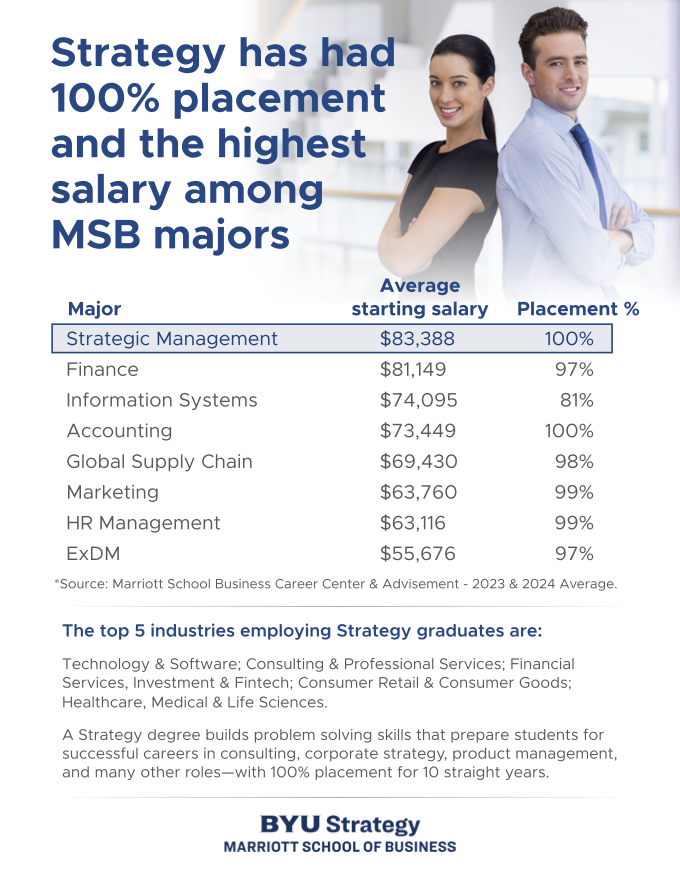
\includegraphics[width=0.65\textwidth,height=\textheight]{images/BYUStrategy-Placement-25.png}
\end{center}

For students looking to go into consulting the Strategy major continues
to have place \textbf{highest number of students at
\href{https://byu-my.sharepoint.com/:b:/g/personal/murff_byu_edu/EXAQsKD1LS5Pm8VckCiUU4gBE9NLnEU2Oieu1exM-GKkUA?e=BxObQe}{MBB
and other top consulting firms}}.

\begin{center}
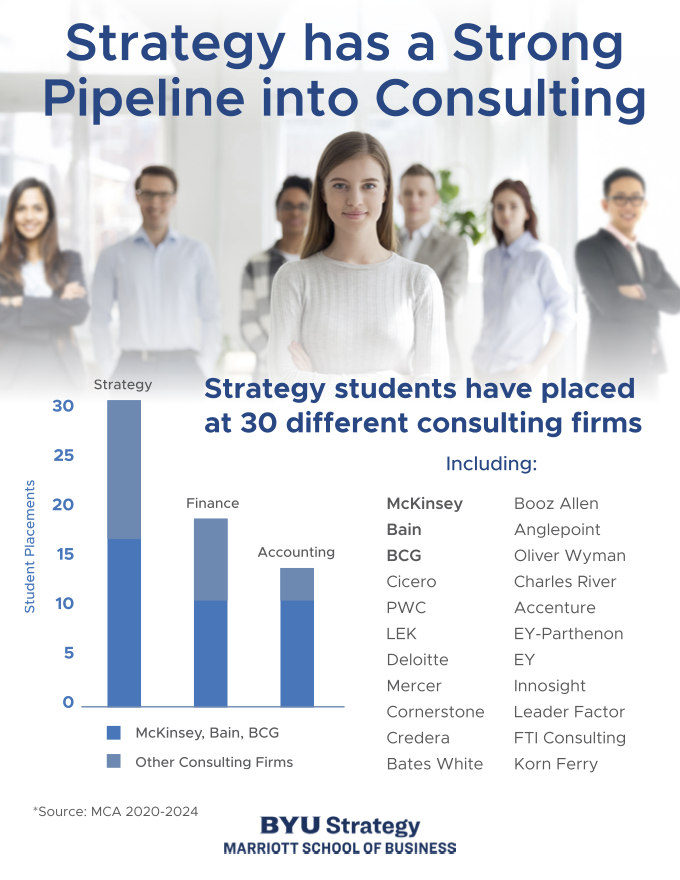
\includegraphics[width=0.65\textwidth,height=\textheight]{images/BYUStrategy-Pipeline-25.pdf}
\end{center}

\section*{What we look for in
applicants}\label{what-we-look-for-in-applicants}
\addcontentsline{toc}{section}{What we look for in applicants}

\markright{What we look for in applicants}

Students who thrive in Strategy tend to be multi-dimensional: strong
academically, good communicators, naturally curious, collaborative with
others, and logical thinkers.

The program is not the best fit for students who prefer highly scripted
and formulaic environments or curriculum.

\section*{Course List}\label{course-list}
\addcontentsline{toc}{section}{Course List}

\markright{Course List}

A list of courses and key questions addressed in each is shown in the
table below:

Course Number

Title

Key Question Addressed by the Class

STRAT 401

Intro to Strategic Management

How do firms sustain competitive advantage and capture value? (case
discussions)

STRAT 402

Economics of Strategy

What are the economic foundations that drive the success and failure of
companies (e.g.~competition, pricing, supply, demand, production, cost)?

STRAT 411

Competitive Strategy

You play the role of consultant and answer for executives: What should
the company do to improve performance in a competitive and always
changing market? (case presentations)

STRAT 412

Data Analytics for Strategists

What is the data telling me? (gather, analyze, and communicate insights)

STRAT 431/432

Strategic Thinking

How can I apply rigorous thinking to broader, societal questions?

ENT 401

Creativity and Innovation

How do companies innovate and create more value for customers?

STRAT 325

Intro to Management Consulting

How can I best prepare to land the interview, nail it, and then excel in
a Management Consulting job?

STRAT 490R

Creating Digital Products with AI: Strategy \& Prototyping

How can I leverage new AI tools to rapidly test and iterate on new
digital product ideas? (build with AI-assisted coding)

STRAT 490R

Understanding AI: From Foundations to Strategy

How does AI work under the hood and what can I expect and not expect
from it? (explores the math and code)

STRAT 490R

Enterprise Technology Strategy in the Age of AI

How can leaders leverage AI to lead responsible digital transformation
within their company?

STRAT 490R

Advanced Strategy Analytics

How can I apply advanced analytics to real business questions? (python,
statistical methods)

\begin{center}\rule{0.5\linewidth}{0.5pt}\end{center}

{} Junior Core {} Electives

\section*{Application Tips}\label{application-tips}
\addcontentsline{toc}{section}{Application Tips}

\markright{Application Tips}

\subsection*{Case preparation}\label{case-preparation}
\addcontentsline{toc}{subsection}{Case preparation}

Your application will include responding to a case question. Answering a
case question is a type of simulation that explores how would would
think through a real business problem. You're asked to analyze a
situation, structure your thinking, and recommend a course of action. It
tests how you break down complex problems, use data, and communicate
solutions clearly and logically while under a bit of time pressure. It's
less about getting the ``exact right answer'' and more about
demonstrating your approach to solving complex, ambiguous problems like
those faced in real life business situations.

You are strongly encouraged to practice several cases before you
complete your actual case interview.

Below you will find two types of case questions both of which will be
valuable to practice. The first two are past case questions from
strategy admissions and the remainder are example cases from McKinsey
and Company.

\href{https://byu-my.sharepoint.com/:w:/g/personal/murff_byu_edu/EYJXiOSdEslHqYeG5AQBLCQB21i0E1blVlS48a0T_oNxMQ?e=IrkYKv}{2023
case qustion and solution}

\href{https://byu-my.sharepoint.com/:w:/g/personal/murff_byu_edu/EY6gqE3YuhJBtc-IEHaNkbIBfsxePrwVqdYbLnxVnIS5dA?e=EeDaUA}{2024
case qustion and solution}

The McKinsey cases are designed for 20 to 30 minute interviews so will
be more involved than what you will have to answer in your application.
If you do well on the McKinsey practice cases, you will likely do well
on the strategy admission case.

\href{https://www.mckinsey.com/careers/interviewing/diconsa}{Deliver
financial services to the unbanked}

\href{https://www.mckinsey.com/careers/interviewing/national-education}{Transform
a national education system}

\href{https://www.mckinsey.com/careers/interviewing/talbot-trucks}{Assess
the feasibility of manufacturing electric trucks}

\href{https://www.mckinsey.com/careers/interviewing/electrolight}{Launch
a new sports drink}




\end{document}
